%!TEX root = ../thesis.tex

\chapter{Results}
\label{chp:results}

This section will cover the results of the verification process as it was described in section \ref{sec:sum-background}.
The main finding is that there are eight assumptions which in total grant that the properties as described in section \ref{sec:ifc-properties} cannot be violated, in other words: the MINRV8 architecture models the information flow properties introduced in this thesis, namely \smv{MEMORY_OP_INTEGRITY}, \smv{CSR_INTEGRITY} and \smv{NO_LEAK}, if and only if the eight assumptions that will be introduced in subsequent sections are in place.

Additionally, roughly 23 bug fix patches\footnote{%
    The number of 23 bug fix patches was measured by counting the amount of patches containing the word \enquote{fix} in its description and being applied to the model file.
} were applied to the model and some \smv{INIT} constraints were set up.
Taken together with aforementioned assumptions these patches mark a fixpoint of the prove-refine loop discussed in section \ref{sec:sum-background} and depicted in figure \ref{fig:ver-process}.

This section is grouped as follows: section \ref{sec:assumptions} will introduce aforementioned assumptions and \smv{INIT} constraints.

Note that only assumptions and no architectural refinements were introduced to the model\footnote{%
    It was tested whether two assumptions could be replaced by one architectural mitigation.
    It turned out, that this architectural refinement did not manage to rule out the respective vulnerability.
    This is discussed at the end of appendix \ref{app:cexs}.
}.
It therefore was also tested how the results would change when canaries are introduced to the architecture.
The term \enquote{canary} refers to birds historically used in coal mines to indicate a loss of oxygen.
In the field of software development, this term refers to bugs that are added to code bases deliberately to test detection mechanisms.
These canaries mimic known vulnerabilities to real-world architectures and will therefore also give an overview of the capabilities of the verification approach of this thesis.
The results of these tests will finally be presented in section \ref{sec:canaries}.

\section{Assumptions}
\label{sec:assumptions}

Technically, \smv{INIT} constraints and assumptions serve the same purpose: They limit the state spaces that will be searched for property violations.
Conceptually, however, these two concepts should be distinguished.
In the model, \smv{INIT} constraints are used to limit the search of the state space to \textit{valid} counter-examples only.
Validity in this context means, that properties are not false to begin with and that the initial state of the architecture complies with the specification.
Consequently, these constraints were introduced during the prove-refine loop as fixes to the model.
Assumptions on the other hand are not part of the model in a technical sense but mark a result of the verification of the architecture: Each assumptions constitutes a rule for e.g., \gls{os} or compiler engineers to obey in order to write or generate non-vulnerable code.

\subsection{Initial Constraints}

Validity of the counter-examples was guaranteed by 13 \smv{INIT} constraints that can be grouped into four categories.
Firstly, two groups of constraints guarantee that counter-examples are not false upfront.
By constraining the contents of registers to only contain confidential data when the architecture starts in machine-mode and to only contain malicious data when the architecture starts in user-mode.
Furthermore, cache and memory can only contain confidential data if the respective memory region is set to \textit{not} be readable for user-mode and can only contain malicious data if the respective memory region \textit{is} set to be writable by user-mode.
For example, assume, the model would not be constrained to initially only contain confidential data in some register when in machine-mode.
In this case, nuXmv returns a trivial counter-example violating the \smv{NO_LEAK} property (\ref{itm:prop-no-leak}) where the architecture starts in user-mode and has confidential data in some register.

Secondly, two more groups of constraints ensures the initial state to comply with the specification is guaranteed.
The first is rather simple, given by a single constraint and depicted in the following snippet:
\begin{lstlisting}[
    language=smv,
    caption={\gls{mstatus} \smv{INIT} constraint for the model}
]
    INIT MIE = 0b_1 -> MPP = 0b_0;
\end{lstlisting}
This constraint ensures that the interrupt handling mechanisms are set up correctly as mandated by the RISC-V specification (cf. section \ref{sec:rv-priv-arch} and figure \ref{fig:interrupt-handling}).
As \smv{MPP} is cleared on return from a trap handler and \smv{MIE} being high implies that no interrupt is being handled at the moment, \smv{MPP} must be low.

The last group of constraints sets up caching errorless, i.e. if the cache is valid, it can only point to an address of a region that is cacheable and must match that addresses content unless the respective region is set to be write-back-cacheable.

\subsection{Property Assumptions}

\begin{table}
    \centering
    \begin{tabular}{| c r | c | c | c |}
        \multicolumn{1}{r}{} & \multicolumn{1}{r}{} &
        \multicolumn{1}{l}{\tilthdr{\smv{MEMORY_OP_INTEGRITY} (\ref{itm:prop-mem-i})}} &
        \multicolumn{1}{l}{\tilthdr{\smv{CSR_INTEGRITY} (\ref{itm:prop-csr-i})}} &
        \multicolumn{1}{l}{\tilthdr{\smv{NO_LEAK} (\ref{itm:prop-no-leak})}} \\
        \hline % \cline{3-5}
        \multirow{2}{*}{Mode-boundary} & \smv{SAN_ON_CALL} & \checkmark & \checkmark & \\
        \cline{3-5}
        & \smv{CLR_ON_RET} &&& \checkmark \\
        \hline % \cline{3-5}
        \multirow{2}{*}{Memory} & \smv{NO_PUBLIC_READS} & \checkmark & \checkmark & \\
        \cline{3-5}
        & \smv{NO_PUBLIC_WRITES} &&& \checkmark \\
        \hline % \cline{3-5}
        \multirow{4}{*}{Memory privilege} & \smv{SAN_ON_CLASSIFICATION} & \checkmark & \checkmark & \\
        \cline{3-5}
        & \smv{CLR_ON_DECLASSIFICATION} &&& \checkmark \\
        \cline{3-5}
        & \smv{SAN_CACHE_ON_CLASSIFICATION} & \checkmark & \checkmark & \\
        \cline{3-5}
        & \smv{CLR_CACHE_ON_DECLASSIFICATION} &&& \checkmark \\
        \hline % \cline{3-5}
    \end{tabular}
    \caption{Assumptions Compared to Properties}
    \label{tbl:assumptions-overview}
\end{table}

During the prove-refine loop, whenever it was found that a counter-example to a property reported by nuXmv was valid and not an actual vulnerability of the architecture but a risk to be controlled by software, an assumption was phrased resembling a mitigation of the respective vulnerability.
This led to a total number of eight assumptions which in total grant the absence of any information flow control violation.
These assumptions can be grouped into three categories:
\begin{itemize}
    \item Mode-boundary crossing related assumptions
    \item Memory related assumptions
    \item Memory privilege related assumptions
\end{itemize}

Find an overview of all these assumptions in table \ref{tbl:assumptions-overview}.
Each row represents one assumption and each column one property.
A check mark denotes that the respective assumption is critical for the respective property, i.e. there exists a counter-example proving the property to be false if the assumption at hand is not assumed.
These counter-examples are given in detail in appendix \ref{app:cexs} and will be skipped here.

Note that each of the assumptions is critical for at least one property.
This shows that \enquote{$ \text{assumptions} \Leftrightarrow \text{properties} $} as opposed to only \enquote{$ \text{assumptions} \Rightarrow \text{properties} $} since \enquote{$ \neg \text{assumptions} \Rightarrow \neg \text{properties} $}.

\paragraph{Mode-boundary crossing related assumptions}
As can be seen in table \ref{tbl:assumptions-overview}, there are two properties related to mode-boundary crossing.
Mode-boundary crossing related here refers to vulnerabilities that violate a property at execution of the \smv{Ecall} or \smv{Mret} instruction.

The first of these is called \smv{SAN_ON_CALL} and mandates from machine-mode to not use \textit{dangerous} instructions before having cleared the registers from any untrusted data when entering machine- from user-mode.
Dangerous instructions here are \minrv{Load}, \minrv{Store}, \minrv{Csrrs} and \minrv{Csrrc} and directly stem from the instructions used in properties \smv{MEMORY_OP_INTEGRITY} (\ref{itm:prop-mem-i}) and \smv{CSR_INTEGRITY} (\ref{itm:prop-csr-i}).
The next assumption to be introduced is called \smv{CLR_ON_RET}; it states: Whenever machine-mode hands back control to user-mode, the registers must be cleared of any confidential information.
The implementation of \smv{SAN_ON_CALL} and \smv{CLR_ON_RET} can be found in snippet \ref{snpt:san-on-call} and \ref{snpt:clr-on-ret} respectively.

Taken together, these two assumptions ensure that machine-mode neither directly hands secrets to nor directly is handed malicious data by user-mode.

\begin{figure}
    \begin{lstlisting}[
        language=smv,
        caption={Assumption \lstinline{SAN_ON_CALL}},
        label={snpt:san-on-call}
    ]
        G (!priv & X priv -> X (
            (priv -> !(op in { LOAD, STORE, CSRRS, CSRRC }))
            U (regs_integrity[0] = 0h_FF
                & regs_integrity[1] = 0h_FF
                & regs_integrity[2] = 0h_FF
                & regs_integrity[3] = 0h_FF)
        ))
    \end{lstlisting}

    \begin{lstlisting}[
        language=smv,
        caption={Assumption \smv{CLR_ON_RET}},
        label={snpt:clr-on-ret}
    ]
        G (
            priv & X !priv -> regs_conf[0] = 0h_00
                & regs_conf[1] = 0h_00
                & regs_conf[2] = 0h_00
                & regs_conf[3] = 0h_00
        )
    \end{lstlisting}
\end{figure}

Both assumptions \smv{SAN_ON_CALL} and \smv{CLR_ON_RET} are similar to each other.
Both were introduced under the label of being \textit{mode-boundary crossing related}, which means that both assumptions are about information flow tracking labels when changing privilege mode - more precisely: both are about the labels of register contents.
The relation of these two assumptions, however, also characterizes a pattern that can also be recognized for subsequent groups of assumptions.
It turned out that for every integrity related assumption, such as \smv{SAN_ON_CALL}, there was a similar confidentiality related assumption such as \smv{CLR_ON_RET}.
This can be seen easily in table \ref{tbl:assumptions-overview}.
In alternating rows, two groups of assumptions can be distinguished: those which are relevant to the properties \smv{MEMORY_OP_INTEGRITY} and \smv{CSR_INTEGRITY} and those which are relevant to the property \smv{NO_LEAK}.
It is noteworthy that these two groups of assumptions can be characterized by the way they constrain information flow which align perfectly with the intuition of the two types of labels:
Confidentiality is about machine-mode not handing out secrets to user-mode, integrity is about user-mode not gaining control over machine-mode.
Consequently, whereas confidentiality related assumptions always constrain flow of information going \textit{out of} machine-mode, integrity related assumptions always constrain flow of information going \textit{into} machine-mode.

\paragraph{Memory related assumptions}
Two assumptions about memory reads and writes join the ranks of these groups, namely \smv{NO_PUBLIC_READS} and \smv{NO_PUBLIC_WRITES} which are formally given in snippet \ref{snpt:no-public-reads} and \ref{snpt:no-public-writes} respectively.
These two assumptions express exactly what the title says; they require machine-mode to never read from or write to public memory.
As such, they directly extend the mode-boundary related assumptions.
At first, it was ensured that machine-mode neither hands out secrets nor accepts malicious data directly.
These two assumptions now ensure that the same must not happen by a detour into memory.

\begin{figure}
    \begin{lstlisting}[
        language=smv,
        caption={Assumption \lstinline{NO_PUBLIC_READS}},
        label={snpt:no-public-reads}
    ]
        G (priv & op = LOAD -> (
            mem_addr < $REGION0_SIZE
                ? !pmpcfg0.write
                : !pmpcfg1.write
        ))
    \end{lstlisting}

    \begin{lstlisting}[
        language=smv,
        caption={Assumption \lstinline{NO_PUBLIC_WRITES}},
        label={snpt:no-public-writes}
    ]
        G (priv & op = STORE -> (
            mem_addr < $REGION0_SIZE
                ? !pmpcfg0.read
                : !pmpcfg1.read
        ))
    \end{lstlisting}
\end{figure}

\paragraph{Memory privilege related assumptions}
The four assumptions that have been introduced up to this point seem to cover all relevant channels of information transmission: registers and memory.
However, these are not enough to ensure that the MINRV8 architecture implements all information flow properties subject to this thesis.
Whereas the two memory related properties covered the group of actions by machine-mode where information directly is given to or taken from user-mode, it is also possible to transmit information indirectly via memory by writing it to or reading it from safe memory regions but then changing the attributes of respective memory regions.
The two assumptions \smv{SANITIZE_ON_DECLASSIFICATION} and \smv{CLR_ON_DECLASSIFICATION} counter issues arising from these vectors.
The former assumption demands from machine-mode to ensure that a memory region does not contain malicious information when it is set to be publicly inaccessible.
This assumption is formalized in snippet \ref{snpt:san-on-classify}.
The latter demands from machine-mode to always ensure that a memory region does not contain confidential information when its made publicly accessible.
This assumption is formalized in snippet \ref{snpt:clr-on-declassify}.

\begin{figure}
    \begin{lstlisting}[
        language=smv,
        caption={Assumption \lstinline{SAN_ON_CLASSIFICATION}},
        label={snpt:san-on-classify}
    ]
        G (pmpcfg0.write & X !pmpcfg0.write
            -> memory_integrity[0] = 0h_FF
             & memory_integrity[1] = 0h_FF)
        & G (pmpcfg1.write & X !pmpcfg1.write
            -> memory_integrity[2] = 0h_FF
             & memory_integrity[3] = 0h_FF)
    \end{lstlisting}

    \begin{lstlisting}[
        language=smv,
        caption={Assumption \lstinline{CLR_ON_DECLASSIFICATION}},
        label={snpt:clr-on-declassify}
    ]
        G (!pmpcfg0.read & X pmpcfg0.read
            -> memory_conf[0] = 0h_00
             & memory_conf[1] = 0h_00)
        & G (!pmpcfg1.read & X pmpcfg1.read
            -> memory_conf[2] = 0h_00
             & memory_conf[3] = 0h_00)
    \end{lstlisting}
\end{figure}

Yet, these two assumptions still not suffice to grant the absence of memory privilege related property counter-examples.
It turns out that only ensuring memory regions to not contain confidential/malicious words when (de-)classifying respective regions allows problematic data to remain in cache which bypasses \smv{SAN_ON_CLASSIFICATION} and \smv{CLR_ON_DECLASSIFICATION}.
This brings the need to also assume that the cache is cleared and sanitized by the architecture whenever a memory region is (de-)classified.
This is expressed in the assumptions \smv{SAN_CACHE_ON_CLASSIFICATION} and \smv{CLR_CACHE_ON_DECLASSFICATION} (cf. snippets \ref{snpt:sanc-on-classify}, \ref{snpt:clrc-on-declassify}).

To summarize all assumptions:
At first, \smv{SAN_ON_CALL} and \smv{CLR_ON_RET} assumed that no direct flow of sensitive or malicious data is possible between user- and machine-mode (snippets \ref{snpt:san-on-call} and \ref{snpt:clr-on-ret}).
Then, these assumptions were generalized to rule out detours into memory by \smv{NO_PUBLIC_WRITES} and \smv{NO_PUBLIC_READS} (snippets \ref{snpt:no-public-writes} and \ref{snpt:no-public-reads}).
Finally, it was assumed that machine-mode must not freely alter access privileges of memory regions.
It must clear or sanitize regions accordingly, depending on the previous access privileges, e.g., machine-mode must ensure to not forget secrets in memory that is made publicly accessible.

\begin{figure}
    \begin{lstlisting}[
        language=smv,
        caption={Assumption \lstinline{SAN_CACHE_ON_CLASSIFICATION}},
        label={snpt:sanc-on-classify}
    ]
        G (pmpcfg0.write & X !pmpcfg0.write
                & cache.valid & cache.addr < $REGION0_SIZE
            -> cache.integrity = 0h_FF) &
        G (pmpcfg1.write & X !pmpcfg1.write
                & cache.valid & $REGION0_SIZE <= cache.addr
            -> cache.integrity = 0h_FF)
    \end{lstlisting}

    \begin{lstlisting}[
        language=smv,
        caption={Assumption \lstinline{CLR_CACHE_ON_DECLASSIFICATION}},
        label={snpt:clrc-on-declassify}
    ]
        G (!pmpcfg0.read & X pmpcfg0.read
                & cache.valid & cache.addr < $REGION0_SIZE
            -> cache.conf = 0h_00) &
        G (!pmpcfg1.read & X pmpcfg1.read
                & cache.valid & $REGION0_SIZE <= cache.addr
            -> cache.conf = 0h_00)
    \end{lstlisting}
\end{figure}

\section{Canaries}
\label{sec:canaries}

In this section, it will be presented how the model of the MINRV8 architecture was altered in order to implement real-world attacks to the Intel x86 architecture.
By default, the MINRV8 architecture is not vulnerable to these attacks, however, making the architecture vulnerable will put the approach of this thesis to formally verify an instruction set architecture to a test.

\subsection{Cache Poisoning Attack on x86}
\label{sec:cache-poisoning}

The cache poisoning attack\footnote{%
    The name \enquote{cache poisoning attack} is not official.
} was discovered and presented by Rafal Wojtczuk and Joanna Rutkowska in their publication \textit{Attacking SMM Memory via Intel CPU Cache Poisoning} \cite{Wojtczuk09}.
\enquote{SMM memory} refers to a specific region of memory that is designed to be only accessible by the mode of highest privilege in x86 architectures: System Management Mode.
This memory is intended to be written only on start-up and then locked down for later write-accesses.
Wojtczuk and Rutkowska, however, managed to find a vulnerability to the x86 architecture which allowed them to effectively write to SMM memory without SMM privileges by marking respective memory region as write-back-cacheable.
The attack comprises the following steps and requires administrator privileges on the machine to be attacked:
\begin{enumerate}
    \item Mark SMM memory as write-back-cacheable using administrator privileges
    \item \label{itm:cache-pois-mem}
    Generate write accesses to the memory.
    Since the region is marked as write-back-cacheable, the writes will not be propagated to the memory controller which would drop these accesses but will be cached.
    \item \label{itm:cache-pois-smi}
    Trigger an System Management Interrupt to transfer control to System Management Mode.
    Depending on the specific addresses written System Management Mode will now execute code written with administrator privileges in step \ref{itm:cache-pois-mem}.
\end{enumerate}

Steps \ref{itm:cache-pois-mem} and \ref{itm:cache-pois-smi} can also be swapped to read from SMM memory.
Then, triggering the interrupt will make SMM mode execute parts of SMM memory which will leave some parts of the handler being cached.
After SMM returns from handling the interrupt, administrator mode can read these words from cache.

This attack does not fully apply to the MINRV8 architecture since it does not support as fine grained privilege modes as the x86 architecture.
In x86, administrator privileges are needed to set SMM memory cacheable and attack SMM-mode which is of higher privilege than administrator-mode.
To apply this attack to the MINRV8 would bring the need of user-mode being able to set cacheability properties of memory regions.
It is not reasonable to assume that anyone would give user-mode this power.
However, the basic idea can still be implemented by following changes to the model:
\begin{itemize}
    \item For all cache transition relations, do not check whether current privilege mode suffices for the memory operation at hand, i.e. user-mode can write to cache of memory regions not set as writable to it.
    \item For load accesses to memory, do not check whether current privilege mode suffices for the memory read if the address is being cached, i.e. user-mode can read cached memory regions even if they're not set as readable to it.
\end{itemize}

These changes manage to introduce a vulnerability to the MINRV8 architecture.
If assuming all assumptions introduced in section \ref{sec:assumptions}, nuXmv manages to find a counter-example for all three information flow properties.
These, again, are discussed in the appendix (cf. \ref{sec:cexs-cache-vuln}).

One distinction from the original cache-poisoning attack to the adaption that has been implemented is that the attacker cannot set the attacked memory region to be cacheable in the first place since user-mode lacks the capabilities to do so.
This difference does not play a major role since the attack can take place nonetheless if some memory region happens to be locked down to user-mode and is set to be write-back-cacheable, this still weakens the attack to some degree.

What can be done to mitigate this attack?
Obviously, the vulnerability purposefully introduced to the architecture could be dropped.
At this point, though, it is not clear how realistic this characteristic of the MINRV8 architecture is since at least in the case of the x86 architecture, the findings of \cite{Wojtczuk09} suggest hardware does not perform privilege checks when writing to the cache.

It not likely, however, that RISC-V is vulnerable to this attack.
One the one hand, the specification states that cacheability settings can be modified by machine-mode only \cite[p.43]{RiscVISAP}.
One the other hand, it also states that \gls{pmp} attributes (including access privileges) are checked in \textit{parallel} to \glspl{pma} (defining cacheability), i.e. regardless of cacheability settings, and always trap at privilege violations \cite[44-45]{RiscVISAP}.
This indicates that neither would a privilege mode other than machine-mode be able to set any memory region cacheable nor would it be able to read from cache of memory regions it otherwise does not have access to.
It should be part of future work, though, to implement a complete model of the RISC-V specification which would verify whether RISC-V is actually not susceptible to this attack vector.

\subsection{The SYSRET Vulnerability}
\label{sec:sysret}

The so called \textit{SYSRET vulnerability} to the intel x86 architecture is listed as vulnerability \textit{CVE-2012-0217} by the \textit{Common Vulnerabilities and Exposures} database (CVE\textsuperscript{\textregistered}) \cite{SYSRET-vuln} and allegedly has also been found by Rafal Wojtczuk \cite{SYSRETFreeBSD,SYSRETDebian,SYSRETCert}.
To our knowledge, the most concise and freely available explanation of the vulnerability can be found in the blog post \textit{The Intel SYSRET Privilege Escalation} by George Dunlap published on the page of Xen Project, a community for virtualization-related open source projects which in part also have been affected by said vulnerability \cite{Dunlap19}.

The x86 architecture provides multiple ways to switch between privilege modes.
In principle, these ways work analogously to how the MINRV8 architecture changes privilege modes: either an interrupt/exception leads to the privilege escalation or a dedicated instruction is executed that changes privilege mode, e.g., \minrv{Ecall} in case of the MINRV8 architecture.
In general, when changing the privilege mode, the \lstinline{RIP} register, which is the \gls{pc} equivalent for x86 architectures, and the stack-pointer are set to the respective version of the targeted privilege-mode.
The designers of the architecture found that parts of the normal privilege mode changing routines could be left out in some scenarios to improve performance.
One of this routines to be left out was changing the stack-pointer by hardware.
These performance improvements are implemented in the \lstinline{SYSCALL} instruction which makes a cheap transition to high-privilege mode by, for instance, not changing the stack-pointer by hardware.
In consequence, there is the analogous \lstinline{SYSRET} instruction to return control back to user-mode which also does not set the stack-pointer.
However, if an interrupt handler invoked by the \lstinline{SYSCALL} instruction intends to use the stack-pointer, it must first set the stack-pointer up accordingly and afterwards set it back to user-mode\footnote{%
    There are more than two privilege modes provided by the x86 architecture and they also have different names than the privilege modes of the MINRV8 architecture, however, the SYSRET vulnerability only touches two privilege modes which have the same purpose as user- and machine-mode of the MINRV8 architecture.
    Therefore, in this context, the terms user-mode and machine-mode can also be used to talk about the x86 architecture.
} before executing the \lstinline{SYSRET} instruction.

When \lstinline{SYSRET} restores the user-mode's context, it reads the \lstinline{RIP} value from the \lstinline{RCX} register which is used to store the original value of the \lstinline{RIP} register during interrupt handling.
Furthermore, the x86 architecture requires the contents of the \lstinline{RIP} register to be in a special form.
The same requirements are, though, not imposed on the contents of the \lstinline{RCX} register.
If, on executing a \lstinline{SYSRET} instruction on an intel x86 system, the \lstinline{RCX} register contains a malformed value in regards to the requirements of the \lstinline{RIP} register, a general protection fault is generated by the architecture which aborts the transition to user-mode.
It is, however, very likely that at this point the interrupt handler would has already set the stack-pointer back to the user-mode's context leaving the machine-mode with a user-mode controlled stack-pointer.
At the time of disclosure of the SYSRET vulnerability, several major operating systems were affected by it, such as Debian \cite{SYSRETDebian}, FreeBSD \cite{SYSRETFreeBSD} and Microsoft Windows 7 \cite{SYSRETMicrosoft}.

The core of the SYSRET vulnerability is the exception that is being generated during the executing of the \lstinline{SYSRET} instruction and handled before privilege is set back to user-mode but after the stack-pointer has been set to user-mode.

It is noteworthy that the SYSRET vulnerability did not affect the x86 specification of Intel but \glspl{os} incorrectly using the specification.
One could argue that the SYSRET vulnerability was only made possible by poor design decisions by Intel, however, at its core, the SYSRET vulnerability only came to effect because \gls{os} engineers did not have this corner case of the specification in mind when writing interrupt handlers.
This stresses the benefits of this thesis's approach since not only the specification but also software running on it will be verified.
It will turn out that the core of the SYSRET vulnerability will be detected by our approach and that both a mitigation in the architecture and in software can be verified to be successful.

\paragraph{Modification of the MINRV8 Architecture}
This very core of the SYSRET vulnerability can optionally be added to the MINRV8 architecture.
This extension adds three new registers and four instructions to the architecture:
\begin{itemize}
    \item Two stack-pointer registers, \smv{sp[0]} and \smv{sp[1]}
    \item A register to select the active stack-pointer \smv{sp_sel}
    \item An instruction to set the currently active stack-pointer to \minrv{rs1 \% 2}, \minrv{Spsel rs1} (stack-pointer select)
    \item An instruction to set the value of the currently active stack-pointer to the address stored in register \minrv{rs1}, \minrv{Spset rs1} (stack-pointer set)
    \item An instruction to push the value in register \minrv{rs1} onto the stack, \minrv{Push rs1}
    \item An instruction to pop a value from the stack and store it into register \minrv{rd}, \minrv{Pop rd}
\end{itemize}

As can be guessed from the available instructions that deal with the stack, not much automation by hardware is supported.
There are no stack-pointers dedicated to specific privilege-modes.
Consequently, stack-pointers are not automatically switched by hardware on privilege-mode changes.
However, when pushing to or popping from the stack, the stack-pointer automatically is in- or decremented.
Additionally, whenever the stack-pointer is in- or decremented and thereby crosses the boundary of a memory region or the memory as a whole, the architecture also ensures that it wraps around inside its memory region.
It might be a threat to some architectures having the stack-pointer move into unsafe memory regions by repeatedly pushing to or popping from it, yet, this aspect is not relevant to the SYSRET vulnerability which is why it was decided to rule these vulnerabilities out by definition.

In the case of the original SYSRET vulnerability, a specially crafted value must have been placed into a special register to trigger an exception during the \lstinline{SYSRET} instruction.
In case of the MINRV8 architecture, no such special mechanisms are given.
Therefore, the vulnerability can only triggered by an external interrupt but this does not conflict with the core idea of the SYSRET vulnerability.

An \smv{INIT} constraint was added to the model ensuring that when the architecture starts in machine-mode, the currently active stack-pointer points to a memory region that is neither read- nor writable to user-mode.
This, as usual, ensures that the information flow properties are not violated by some obvious initial condition.

Furthermore, with the extension to the architecture comes an assumption that emulates all the major steps that software vulnerable to the SYSRET attack already follows but which do not suffice to implement a secure system.
This assumption is called \smv{SP_BANK} and is depicted in snippet \ref{snpt:sp-bank}.
It comprises four parts.
Firstly, in lines \ref{ln:sp-call-start}-\ref{ln:sp-call-end}, it is assumed that machine-mode must not use the \minrv{Push} or \minrv{Pop} instructions before the stack points to a safe memory region.
Alternatively, machine-mode also might not use these instructions at all until it returns control back to user-mode.
Secondly, in lines \ref{ln:sp-return-start}-\ref{ln:sp-return-end}, whenever machine-mode hands control back to user-mode the prior instruction must have selected a stack-pointer that is user-mode controllable.
This assumption is the most critical to the SYSRET vulnerability.
These two assumptions closely resemble the assumptions \smv{SAN_ON_CALL} and \smv{CLR_ON_RET} as shown in section \ref{sec:assumptions} and snippets \ref{snpt:san-on-call} and \ref{snpt:clr-on-ret} respectively.

Thirdly, in lines \ref{ln:sp-sel-start}-\ref{ln:sp-sel-end}, machine-mode is also not allowed to use the \minrv{Push} or \minrv{Pop} instructions when it \textit{selects} a stack-pointer pointing to a user-mode-controlled region.
This ensures that machine-mode not deliberately decides to use a bad stack-pointer.
And lastly, in lines \ref{ln:sp-set-start}-\ref{ln:sp-set-end}, for the same reasons it is also assumed that machine-mode does not set its stack-pointer to point to a memory region controlled by user-mode.
These two parts follow the same structure as the first part of the \smv{SP_BANK} assumption but trigger on different conditions.

\begin{figure}
    \begin{lstlisting}[
        language=smv,
        caption={Assumption \lstinline{SP_BANK}},
        label={snpt:sp-bank}
    ]
        G (!priv & X priv -> X ( (*\label{ln:sp-call-start}*)
            (priv -> !(op in { PUSH, POP }))
            U ((op = MRET & MPP = 0b_0) | sp[sp_sel] < $REGION0_SIZE
                ? !pmpcfg0.write & !pmpcfg0.read
                : !pmpcfg1.write & !pmpcfg1.read)
        )) & (*\label{ln:sp-call-end}*)
        G (op = MRET -> (sp[sp_sel] < $REGION0_SIZE (*\label{ln:sp-return-start}*)
            ? pmpcfg0.read & pmpcfg0.write
            : pmpcfg1.read & pmpcfg1.write)) & (*\label{ln:sp-return-end}*)
        G (priv & op = SPSEL & (sp[rs1 mod 2] < $REGION0_SIZE (*\label{ln:sp-sel-start}*)
                ? pmpcfg0.write | pmpcfg0.read
                : pmpcfg1.write | pmpcfg1.read)
            -> X (
                (priv -> !(op in { PUSH, POP }))
                U ((op = MRET & MPP = 0b_0) | sp[sp_sel] < $REGION0_SIZE
                    ? !pmpcfg0.write & !pmpcfg0.read
                    : !pmpcfg1.write & !pmpcfg1.read)
            )) & (*\label{ln:sp-sel-end}*)
        G (priv & op = SPSET & (mem_addr < $REGION0_SIZE (*\label{ln:sp-set-start}*)
                ? pmpcfg0.write | pmpcfg0.read
                : pmpcfg1.write | pmpcfg1.read)
            -> X (
                (priv -> !(op in { PUSH, POP }))
                U ((op = MRET & MPP = 0b_0) | sp[sp_sel] < $REGION0_SIZE
                    ? !pmpcfg0.write & !pmpcfg0.read
                    : !pmpcfg1.write & !pmpcfg1.read)
            )) & (*\label{ln:sp-set-end}*)
    \end{lstlisting}
\end{figure}

All these assumptions, however, do not ensure that the architecture models all information flow properties.
Similar to the SYSRET vulnerability, there is a stream of instructions that violates each of these properties which will be discussed in the appendices' section \ref{sec:cexs-sysret}.

\paragraph{Mitigations}

To explore the SYSRET vulnerability in more detail, two approaches to mitigate said vulnerability were tested and added to the model.
One approach lies upon the burden of ensuring security on the programs running on the architecture and is expressed in form of an assumption, the other modifies the architecture and does not rely on on programs to implement certain guidelines.

Aforementioned assumption is depicted in snippet \ref{snpt:sp-safety}.
It states that interrupts must be disabled, whenever machine-mode hands back control to user-mode.
This rules out any attack vector where an external interrupt aborts the execution of the \minrv{Mret} instruction leaving machine-mode with a user-mode-controlled stack pointer.
Some pending external interrupt can then only be handled after the \minrv{Mret} instruction has been executed.
This resembles AMD's version of the x86 architecture which is not susceptible to the SYSRET vulnerability \cite{Dunlap19}.
In AMD's implementation of the x86 architecture, when setting the \lstinline{RIP} with a bad value the general protection fault is thrown after the privilege mode has been lowered rendering the SYSRET attack vector ineffective.

\begin{figure}
    \begin{lstlisting}[
        language=smv,
        caption={Assumption \smv{SP_SAFETY}},
        label={snpt:sp-safety}
    ]
        G (priv & op = MRET & MPP = 0b_0 -> MIE = 0b_0) &
    \end{lstlisting}
\end{figure}

Consider Fedora's mitigation to the SYSRET vulnerability \cite{FedoraSysretMit} as a real-world example.
The interrupt handlers were modified such that if the user could have changed the \lstinline{RIP} value, i.e. might contain an uncanonical value, the \lstinline{IRET} instead of the \lstinline{SYSRET} instruction is used.
This would also be verifiable by our approach: the condition under which \lstinline{IRET} is chosen over \lstinline{SYSRET} would form the antecedent and \smv{op = IRET} the consequent of the implication in snippet \ref{snpt:sp-safety}.
For the MINRV8, however, there is no other choice than disabling interrupts as the source of the \textit{external} interrupt cannot be controlled.

The other mitigation modifies the architecture.
The stack-pointer extension of the MINRV8 architecture was altered such that the two stack-pointers are assigned to privilege-modes and switched by hardware.
Whenever the architecture changes into machine-mode, \smv{sp_sel} is set to 1 and whenever it changes into user-mode \smv{sp_sel} is set to 0.
Furthermore, the \minrv{Spsel} instruction is disabled.
Therefore, with this modification to the architecture the assumptions \smv{SP_BANK} and \smv{SP_SAFETY} can be dropped.
However, new assumptions and \smv{INIT} constraints must be introduced.
With the hardware automatically switching stack-pointers, it must be ensured that the memory regions these stack-pointers point to always are assigned with the respective privileges, i.e. user-mode-stack-pointer is user-mode-read- and -writeable, etc.
This is assumed initially, and made stable by the assumption given in snippet \ref{snpt:sp-autobank-assumption}.
These assumptions are to some extent unrealistic as it cannot be taken for granted that machine-mode actually is capable of setting up the memory regions correctly and guaranteeing that user-mode does not interfere with these settings.
However, verifying such mechanisms does not serve any purpose at this point and was skipped as a consequence.
We therefore make aforementioned assumptions to show that \textit{given} such mechanisms, the herein proposed hardware mitigation to the SYSRET vulnerability can be verified by our approach.

\begin{figure}
    \begin{lstlisting}[
        language=smv,
        caption={Additional assumptions for hardware changes},
        label={snpt:sp-autobank-assumption}
    ]
        G (op != SPSET & (sp[0] < $REGION0_SIZE
                ? pmpcfg0.write & pmpcfg0.read
                : pmpcfg1.write & pmpcfg1.read)
            & (sp[1] < $REGION0_SIZE
                ? !pmpcfg0.write & !pmpcfg0.read
                : !pmpcfg1.write & !pmpcfg1.read)) &
    \end{lstlisting}
\end{figure}

With both stack-pointer related assumptions, \smv{SP_BANK} and \smv{SP_SAFETY}, nuXmv manages to verify that the architecture does not violate integrity information flow properties.
The same is true for the modification of the architecture where the stack-pointer is selected automatically by the architecture and the assumptions \smv{SP_BANK} and \smv{SP_SAFETY} are dropped.

\section{Summary}

In this chapter, the results to the prove-refine loop were presented:
\begin{itemize}
    \item 23 fixes were applied to the model of the MINRV8 architecture,
    \item four categories of \smv{INIT} constraints were set up, and most importantly
    \item eight assumptions were phrased that were verified to grant the absence of information flow property violations.
\end{itemize}

These assumptions are visualized in figure \ref{fig:ifc-assumptions} that again takes inspiration from digital timing diagrams.
The eight assumptions introduced in section \ref{sec:assumptions} constrain streams of instructions to always resemble the following properties:
Whenever machine-mode is called from user-mode by the \minrv{Ecall} instruction or there is an external interrupt, machine-mode must not use memory or \gls{csr} related instructions in the area colored in yellow until some form of a sanitization procedure (\smv{SAN}) has been completed.
This leads to the integrity labels of inputs to these instructions being high after the sanitization procedure.
This property is made stable by the \smv{NO_PULIC_READS} and \smv{SAN_(CACHE)_ON_CLASSIFICATION} assumptions which ensure that no malicious data is loaded from memory or cache as long as machine-mode has control.
If any of these are not assumed, the inputs to memory or \gls{csr} related instructions might become low e.g., somewhere in the orange colored area of the second row.

In general, during execution of a trap handler in machine-mode, confidential data will be handled and therefore, the confidentiality labels of the registers become high at some point.
The \smv{CLR_ON_RET} assumption then enforces that before the \minrv{Mret} instruction is executed by machine-mode to hand back control to user-mode, a procedure to clear the contents of the registers must be executed (\smv{CLR}) after which no other confidential data may be loaded into registers.
This window is colored in green.
The assumptions \smv{NO_PUBLIC_WRITES} and \smv{CLR_(CACHE)_ON_DECLASSIFICATION} again make this property stable after the registers have been cleared and control has been returned to user-mode, leaving it no room to circumvent the clearing of registers.
Again, the orange colored area of the first row shows where user-mode might be able to load secrets from memory or cache if these assumptions were not in place.

\begin{figure}
    \centering
    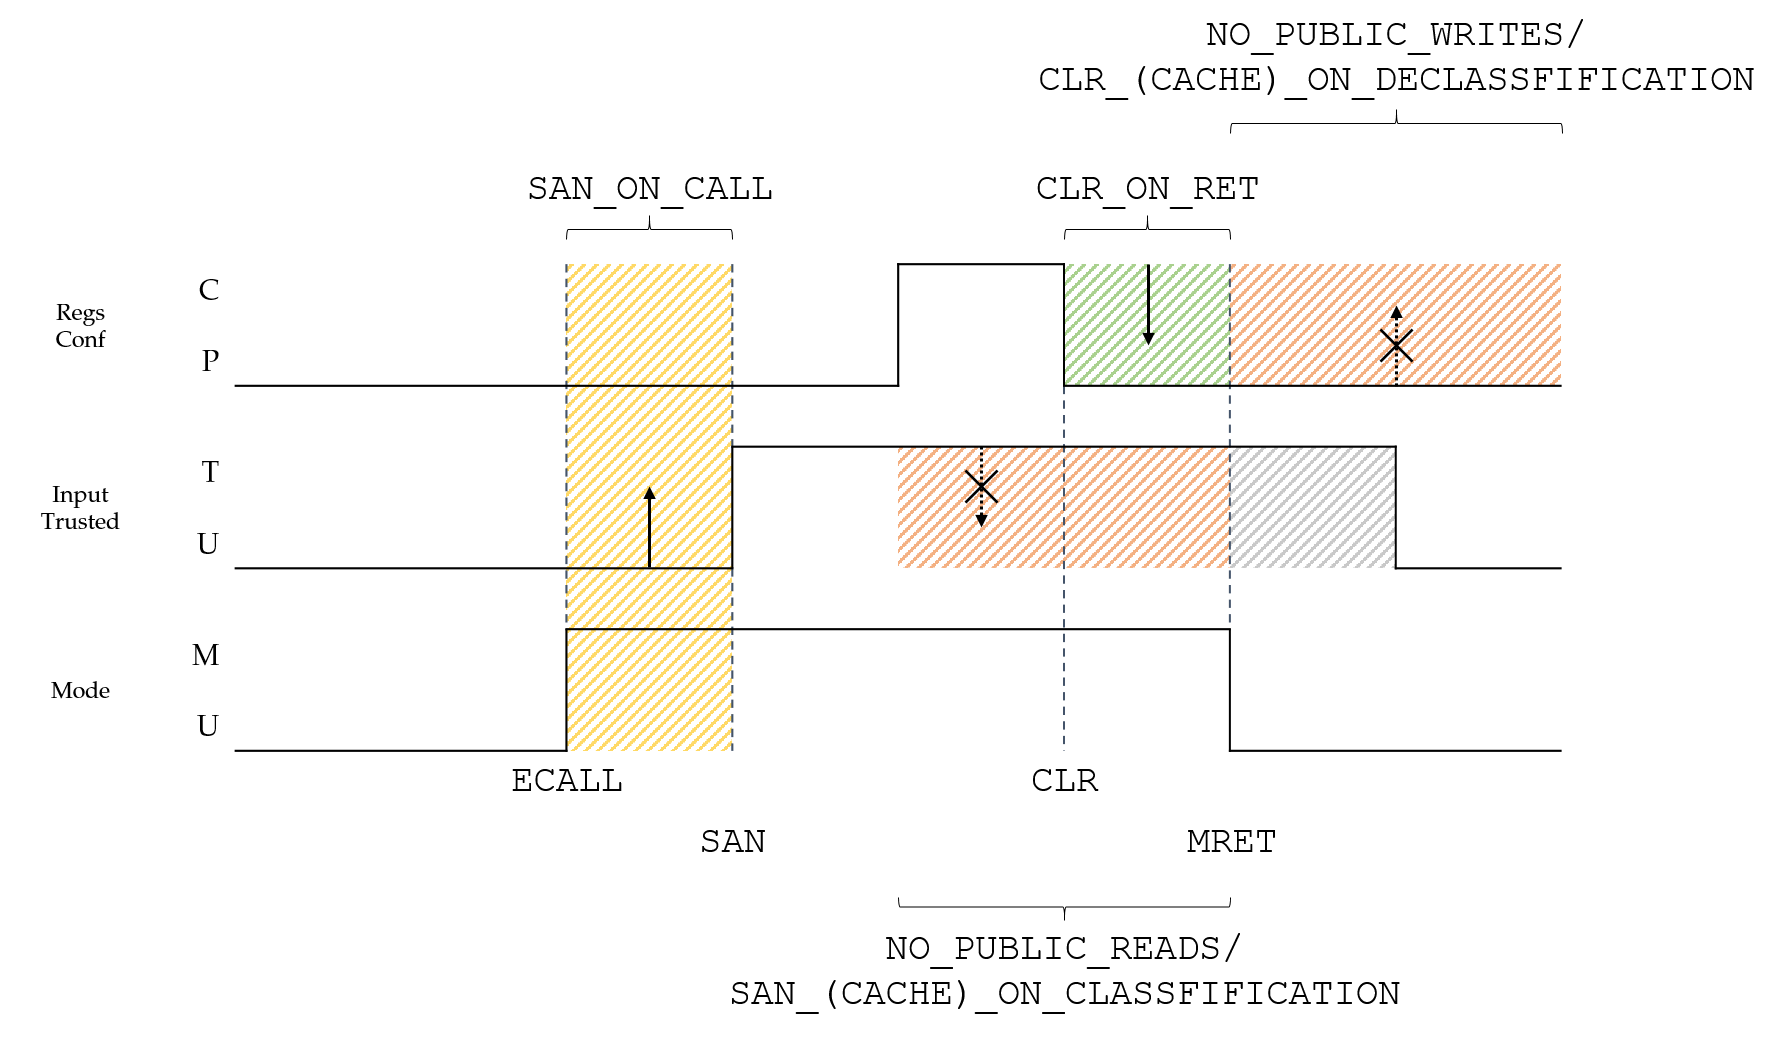
\includegraphics[width=\textwidth]{figures/assumptions.png}
    \caption{Assumptions visualized}
    \label{fig:ifc-assumptions}
\end{figure}

Two aspects were examined to strengthen these assumptions: it was shown that \enquote{assumptions $ \Leftrightarrow $ properties} as not assuming a single one of these leads to the failure of at least one information flow property and two canaries, the deliberate insertion of vulnerabilities into the model, were tested.
It was discussed that it is possible to find both the cache poisoning \cite{Wojtczuk09} and the SYSRET vulnerabilies \cite{SYSRET-vuln,Dunlap19} to the x86 architecture can be modelled such that they apply to a slightly adjusted version of the MINRV8 architecture and can be found without any manual intervention.
The information flow properties and the assumptions did not need to be adjusted such that nuXmv would return a trace illustrating the respective vulnerability.
